\documentclass[11pt,letterpaper]{article}
% PDF reproductible : sans date de compilation ni identifiant aleatoire, pour que git ne voie pas
% de changement quand le contenu est le meme
\pdfinfoomitdate=1
\pdftrailerid{}
\pdfsuppressptexinfo=-1
%graph pour image H
\usepackage{float}

% Pour Dessin
\usepackage{tikz}
\usepackage{amsmath}
\usetikzlibrary{arrows.meta, positioning, patterns, decorations.pathreplacing}

% packetages pour ecrire en français
\usepackage[french]{babel}
\usepackage[utf8]{inputenc}
\usepackage[T1]{fontenc}

% pour les maths, les graphiques et la navigation dans le pdf
\usepackage{amsmath, amssymb, mathtools, bm, array}
\usepackage{graphicx,caption,subcaption}
\graphicspath{{./}}
\usepackage{hyperref}
\hypersetup{
    pdftitle={Vitesse et distance d'une voiture mesurées par effet Doppler},
    pdfauthor={L-F. Brodeur (LFBRO1), S. L-Tremblay (SILAT10)}
}

% marges, police de caractère et header
\usepackage{geometry}
\geometry{top=23mm, bottom=23mm, left=20mm, right=20mm}
\usepackage{cochineal}
\usepackage{fancyhdr}
\pagestyle{fancy}

\parindent=0mm % pas d'indentation

\lhead{L-F. Brodeur (IDUL: LFBRO1) et S. L-Tremblay (IDUL: SILAT10)}
\rhead{Acoustique: effet Doppler d'une voiture}
\fancyheadoffset{0 cm}

\setlength{\headheight}{13.6pt}
\addto\captionsfrench{\renewcommand{\tablename}{Tableau}}

% Bibliographie: une reference n'apparait que si elle est citee dans le texte.
% \cite ecrit \citation{cle} dans le .aux, relu au debut du document a la compilation suivante.
\makeatletter
\def\citation#1{\@for\@clecitee:=#1\do{\expandafter\gdef\csname refcitee@\@clecitee\endcsname{}}}
\newcommand{\refsicitee}[2]{\@ifundefined{refcitee@#1}{}{\bibitem{#1}#2}}
\makeatother

% commandes pour ecrire des equations plus vite avec leur label
\newcommand{\beq}[1]{\begin{equation} \label{#1}}
\def\enq{\end{equation}}

% C'est parti!
\begin{document}
\shorthandoff{;:!?}
\thispagestyle{empty} % pas de header sur la première page
\begin{center}

\noindent
\begin{minipage}[t]{0.5\textwidth}
\raggedright
{\large GPH-3000 \textit{Travaux pratiques avancés}}\\
{\large Automne 2026 $\vert$ GPH-3000 (Groupe: 85213)}
\end{minipage}%
\begin{minipage}[t]{0.5\textwidth}
\raggedleft
{\large \textsc{L-F. Brodeur (IDUL: LFBRO1)}}\\
{\large \textsc{S. L-Tremblay (IDUL: SILAT10)}}
\end{minipage}
\\~\\
\vspace{1em}
{\Large \textbf{Vitesse et distance d'une voiture mesurées par effet Doppler} }\\
[0.3em]
{\large Date du Laboratoire: 12 novembre 2026 \qquad\qquad\qquad Remis le \today}

\end{center}

\vspace{0.5em}
\subsection*{Résumé}
Quand une voiture nous croise, son bruit baisse d'un coup, et la forme de cette baisse dépend de la vitesse de la voiture et de la distance à laquelle elle passe. Dans cette expérience, le système de son d'une voiture jouait un sinus de 440~Hz pendant qu'elle passait en ligne droite devant un sonomètre, à 3,53~m ou à 8,97~m de sa trajectoire, à des vitesses visées entre 10 et 70~km/h. La fréquence reçue a été suivie dans le spectrogramme de chacun des 11 passages, puis un curve fit du modèle Doppler a donné la vitesse et la distance de la voiture. Quand la distance est connue, la vitesse est mesurée avec une incertitude de 0,3 à 6~km/h. À 8,97~m, les vitesses mesurées (de $27{,}1 \pm 0{,}8$ à $62{,}6 \pm 1{,}6~\text{km/h}$ pour 30 à 70~km/h visés) sont entre 6 et 11~\% sous la vitesse visée, ce qui correspond à l'erreur permise pour un compteur de vitesse. À 3,53~m, les passages à 50, 60 et 70~km/h sont plus lents que prévu, probablement parce que la voiture n'a pas roulé à vitesse constante devant le micro. Trouver la distance avec l'audio seulement est plus difficile: à 3,53~m, le curve fit donne des distances entre 1,5 et 5,3~m avec une incertitude d'environ 1~m, et à 8,97~m il ne converge pas pour trois passages sur cinq. La zone de 20~m où la voiture roulait à vitesse constante est trop courte pour séparer la vitesse de la distance. En 1957, deux physiciens de l'Université Johns Hopkins ont résolu le même problème avec le signal radio de Spoutnik: la courbe Doppler d'un seul passage du satellite leur a suffi pour calculer toute son orbite, ce qui a mené au premier système de navigation par satellite \cite{guier}.

\section{Introduction}

Christian Doppler a prédit en 1842 que la fréquence d'une onde change quand la source et l'observateur se déplacent l'un par rapport à l'autre \cite{doppler}. Trois ans plus tard, Buys Ballot a vérifié cette prédiction pour le son près d'Utrecht: des trompettistes jouaient une note fixe sur un train en marche, et des musiciens qui avaient l'oreille absolue notaient la note entendue depuis le quai \cite{buysballot}.

Quand une voiture passe devant nous, la fréquence reçue ne saute pas d'une valeur à l'autre. Elle descend progressivement, et la forme de la courbe dépend de la vitesse de la voiture et de la distance à laquelle elle passe. Il y avait deux objectifs à cette expérience. Premièrement, voir comment la vitesse et la distance changent la courbe de la fréquence en fonction du temps. Deuxièmement, savoir si l'enregistrement d'un seul passage suffit pour retrouver la vitesse et la distance de la voiture.

La Section~\ref{sec:theorie} présente le modèle Doppler pour une source qui passe en ligne droite. La Section~\ref{sec:methodologie} décrit le montage, l'acquisition et l'analyse. Les résultats sont présentés à la Section~\ref{sec:resultats}. Ils sont discutés à la Section~\ref{sec:discussion}. La Section~\ref{sec:conclusion} conclut.

\section{Théorie}
\label{sec:theorie}

On considère une source qui émet une fréquence $f_0$ et qui se déplace en ligne droite à une vitesse constante $v$. Le micro est fixe, à une distance $d$ du point $P$ de la trajectoire qui est le plus proche de lui (Figure~\ref{fig:schema}). On note $x$ la position de la source le long de la trajectoire, avec $x < 0$ avant le point $P$ et $x > 0$ après. Si $\theta$ est l'angle entre la vitesse de la source et la droite qui va de la source au micro au moment de l'émission, le micro reçoit la fréquence \cite{morse}
\beq{eq:doppler}
    f = \frac{f_0}{1 - \dfrac{v}{c}\cos\theta} = \frac{f_0}{1 + \dfrac{v}{c}\,\dfrac{x}{\sqrt{x^2 + d^2}}} ,
\enq
où $c$ est la vitesse du son. Le son émis à la position $x = v\,(t_e - t_p)$, au temps $t_e$, arrive au micro au temps
\beq{eq:retard}
    t = t_e + \frac{\sqrt{x^2 + d^2}}{c} ,
\enq
où $t_p$ est le moment où la source passe au point $P$. Les équations~\ref{eq:doppler} et~\ref{eq:retard} donnent la fréquence reçue $f(t)$ en fonction des trois paramètres $v$, $d$ et $t_p$.

Loin avant le point $P$, $\cos\theta \to 1$ et la fréquence tend vers $f_a = f_0/(1 - v/c)$. Loin après, elle tend vers $f_e = f_0/(1 + v/c)$. La hauteur de la chute de fréquence dépend donc seulement de $v$, et on a $v = c\,(f_a - f_e)/(f_a + f_e)$. Au passage, la fréquence reçue vaut $f_0$ et sa pente est d'environ
\beq{eq:pente}
    \left.\frac{\mathrm{d}f}{\mathrm{d}t}\right|_{x=0} \approx -\frac{f_0\,v^2}{c\,d} .
\enq
La chute dure donc environ $2d/v$: plus la voiture passe loin ou lentement, plus la chute est lente. Pour séparer $v$ et $d$, il faut donc voir la hauteur de la chute et sa durée. Si la vitesse n'est constante que sur une zone $|x| \leq L$, la fréquence n'atteint jamais $f_a$ ou $f_e$: au bord de la zone, $\cos\theta = L/\sqrt{L^2 + d^2}$ seulement.

Finalement, la vitesse du son dans l'air dépend de la température $T$ (en $^\circ$C) \cite{kinsler}:
\beq{eq:c}
    c = 331{,}3\,\sqrt{1 + \frac{T}{273{,}15}}~\text{m/s} .
\enq

\section{Méthodologie}
\label{sec:methodologie}

\subsubsection*{Montage et acquisition}
Les mesures ont été faites le 12 novembre 2026 sur une route droite, à une température d'environ 1~$^\circ$C, ce qui donne $c = 331{,}9~\text{m/s}$ (équation~\ref{eq:c}). Le système de son de la voiture jouait un sinus de 440~Hz pendant tout le passage. Le micro était un sonomètre Piccolo~II placé à $d = 3{,}53~\text{m}$ de la trajectoire, puis 5,44~m plus loin, à $d = 8{,}97~\text{m}$ (Figure~\ref{fig:schema}). Ces distances sont mesurées au ruban jusqu'au côté de la voiture qui fait face au micro. Le fonctionnement d'un sonomètre est décrit dans le protocole du cours \cite{protocole}. Son signal audio brut (44\,117~échantillons par seconde, 16~bits) était lu par USB avec un programme Python écrit par l'équipe et enregistré pour chaque passage.

\begin{figure}[htbp]
    \centering
    \begin{tikzpicture}[scale=0.95, >=Stealth]
        % route et trajectoire
        \fill[gray!15] (-6.5,-1.0) rectangle (6.5,1.0);
        \draw (-6.5,1.0) -- (6.5,1.0);
        \draw (-6.5,-1.0) -- (6.5,-1.0);
        \draw[dashed, gray] (-6.5,0) -- (6.5,0);
        \node[above left, gray!60!black] at (6.5,0) {\small trajectoire};
        % trajet du son (sous la voiture)
        \draw[blue!70!black, thick, ->] (-4.0,0) -- (-0.05,-2.96);
        \node[blue!70!black, below left] at (-2.0,-1.5) {\small son reçu};
        % voiture et vitesse
        \fill[gray!60] (-4.7,-0.45) rectangle (-3.3,0.45);
        \draw (-4.7,-0.45) rectangle (-3.3,0.45);
        \node[below, font=\small] at (-4.15,-0.45) {voiture};
        \draw[->, very thick] (-3.2,0) -- (-2.0,0);
        \node[above] at (-2.1,0.05) {$v$};
        % point P
        \fill (0,0) circle (0.06);
        \node[above right] at (0,0) {$P$};
        % sonometre
        \fill (-0.15,-3.3) -- (0.15,-3.3) -- (0,-3.0) -- cycle;
        \node[below] at (0,-3.3) {sonomètre};
        % angle theta (etiquette sur la bissectrice)
        \draw (-2.7,0) arc (0:-36.87:1.3);
        \node at ({-4.0+1.75*cos(-18.43)},{1.75*sin(-18.43)}) {$\theta$};
        % cote d
        \draw[gray] (0.2,-3.0) -- (1.1,-3.0);
        \draw[<->] (0.9,0) -- (0.9,-3.0) node[midway, right] {$d$};
        % cotes x et zone a vitesse constante: lignes de rappel, puis fleches
        \draw[gray] (-4.0,0.5) -- (-4.0,1.6);
        \draw[gray] (0,0.15) -- (0,2.5);
        \draw[gray] (-5.6,1.05) -- (-5.6,2.5);
        \draw[gray] (5.6,1.05) -- (5.6,2.5);
        \draw[<->] (-4.0,1.4) -- (0,1.4) node[midway, above] {$x$};
        \draw[<->] (-5.6,2.3) -- (0,2.3) node[midway, above] {\small 10~m};
        \draw[<->] (0,2.3) -- (5.6,2.3) node[midway, above] {\small 10~m};
    \end{tikzpicture}
    \caption{Vue de haut du montage (pas à l'échelle). La voiture roulait à vitesse constante sur environ 10~m avant et 10~m après le point $P$, le plus proche du sonomètre.}
    \label{fig:schema}
\end{figure}

Le conducteur visait une vitesse au compteur et la gardait constante sur environ 20~m, soit 10~m avant et 10~m après le point $P$. Avant cette zone, la voiture accélérait, et après, elle freinait. Il y a eu un passage pour chaque vitesse visée: 10, 30, 50, 55, 60 et 70~km/h à 3,53~m, et 10, 30, 50, 60 et 70~km/h à 8,97~m, pour un total de 11 passages.

\subsubsection*{Analyse}
L'analyse a été faite en Python. Le signal est découpé en trames de 4096~échantillons (93~ms) qui avancent de 256~échantillons (5,8~ms). Pour chaque trame, la fréquence du maximum du spectre entre 400 et 485~Hz est trouvée par interpolation entre les canaux de fréquence. Cette bande évite une raie fixe du bruit de fond à 385~Hz. Les trames où le maximum ne dépasse pas le niveau médian de la bande d'au moins 15~dB sont rejetées.

Le modèle des équations~\ref{eq:doppler} et~\ref{eq:retard} est ensuite ajusté à la fréquence en fonction du temps avec un curve fit, avec $f_0 = 440~\text{Hz}$. Le curve fit utilise seulement les points émis dans la zone à vitesse constante ($|x| \leq 10~\text{m}$). La zone est aussi coupée là où la fréquence remonte, parce qu'à vitesse constante la fréquence reçue ne fait que diminuer. Une fréquence qui monte avant le passage indique donc que la voiture accélère encore, et une fréquence qui remonte après le passage indique qu'elle freine. Deux curve fits sont faits pour chaque passage. Dans le premier, $d$ est fixée à la distance mesurée au ruban et le curve fit donne $v$. Dans le deuxième, $d$ est libre, et le curve fit donne $v$ et $d$ à partir de l'audio seulement.

\subsubsection*{Incertitudes}
Les incertitudes du curve fit viennent de sa matrice de covariance. Comme les trames se chevauchent, 16~trames successives partagent les mêmes échantillons et ne sont pas indépendantes. Les incertitudes du curve fit sont donc multipliées par $\sqrt{16} = 4$. Le curve fit donne en fait le rapport $v/c$, donc l'incertitude sur la température ($\Delta T = 1~^\circ\text{C}$, soit $\Delta c = 0{,}6~\text{m/s}$) est propagée dans la vitesse:
\beq{eq:incertitude}
    \Delta v = \sqrt{\left(\Delta v_{\text{fit}}\right)^2 + \left(\frac{\partial v}{\partial c}\,\Delta c\right)^2} = \sqrt{\left(\Delta v_{\text{fit}}\right)^2 + \left(\frac{v}{c}\,\Delta c\right)^2} .
\enq
Le deuxième terme ne vaut que 0,2~\% de $v$, donc l'incertitude vient presque entièrement du curve fit.

\section{Résultats}
\label{sec:resultats}

La Figure~\ref{fig:spectro} montre le spectrogramme de deux passages à 50~km/h. Avant le passage, la raie du sinus est autour de 457~Hz, et après le passage, elle est autour de 430~Hz. À 8,97~m, la chute est visiblement plus lente qu'à 3,53~m. On voit aussi une bande verticale de bruit large bande autour du passage (bruit du moteur et des pneus), plus forte à 3,53~m, ainsi que la raie fixe à 385~Hz.

\begin{figure}[htbp]
    \centering
    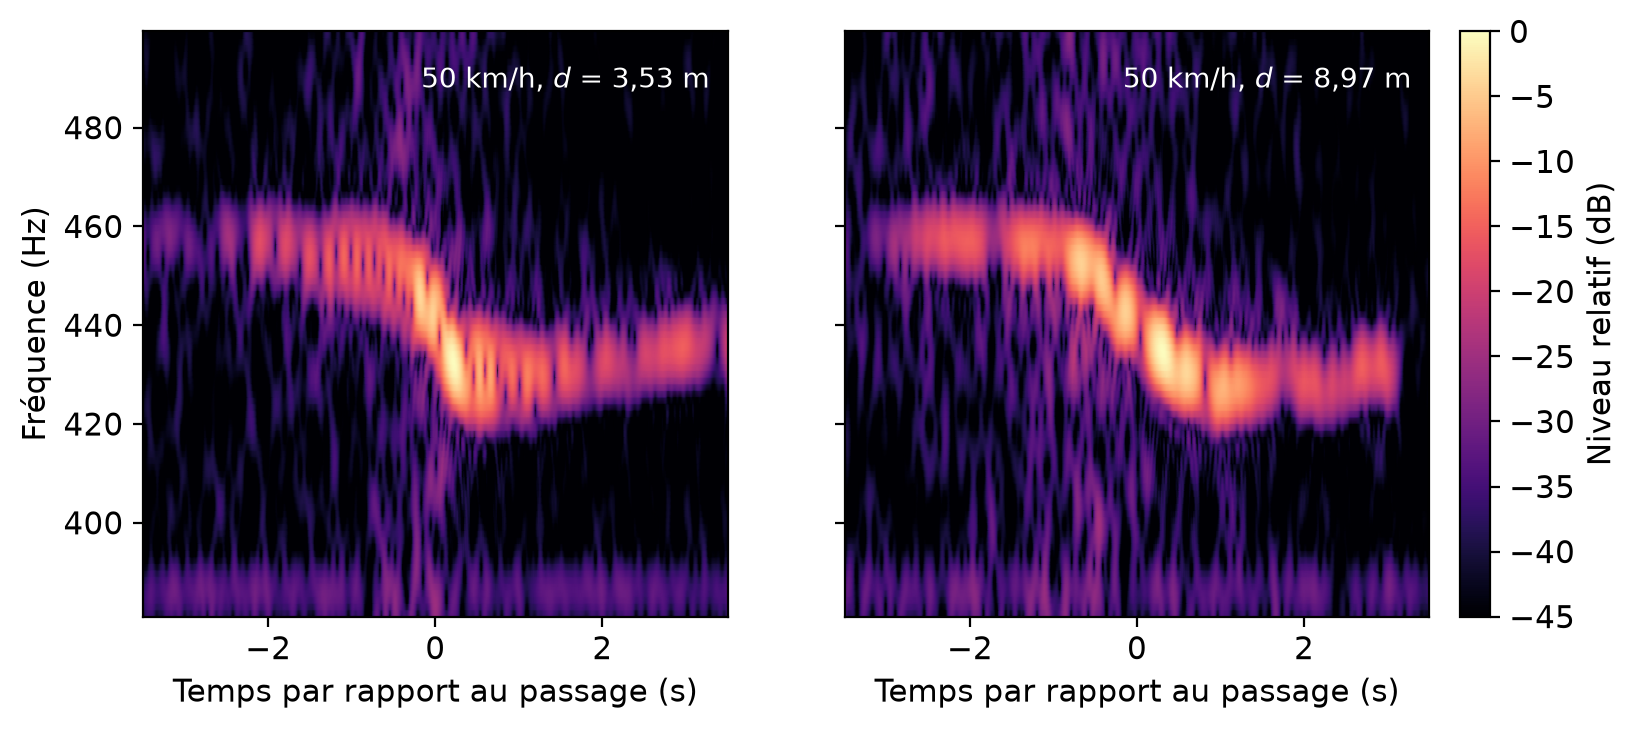
\includegraphics[width=0.8\textwidth]{../figures/01_spectrogrammes.png}
    \caption{Spectrogrammes de deux passages à 50~km/h visés, à 3,53~m (gauche) et à 8,97~m (droite) de la trajectoire. La chute de fréquence dure environ 0,7~s à 3,53~m et environ 1,5~s à 8,97~m.}
    \label{fig:spectro}
\end{figure}

La Figure~\ref{fig:courbes} montre la fréquence suivie dans la zone à vitesse constante pour les 11 passages, avec le curve fit où $d$ est fixée. Plus la vitesse est grande, plus la chute est haute. À la même vitesse, la chute est plus lente à 8,97~m, comme le prévoit l'équation~\ref{eq:pente}. L'écart quadratique moyen entre les points et le curve fit est de 1,0 à 1,6~Hz à 8,97~m et de 0,7 à 3,0~Hz à 3,53~m.

\begin{figure}[htbp]
    \centering
    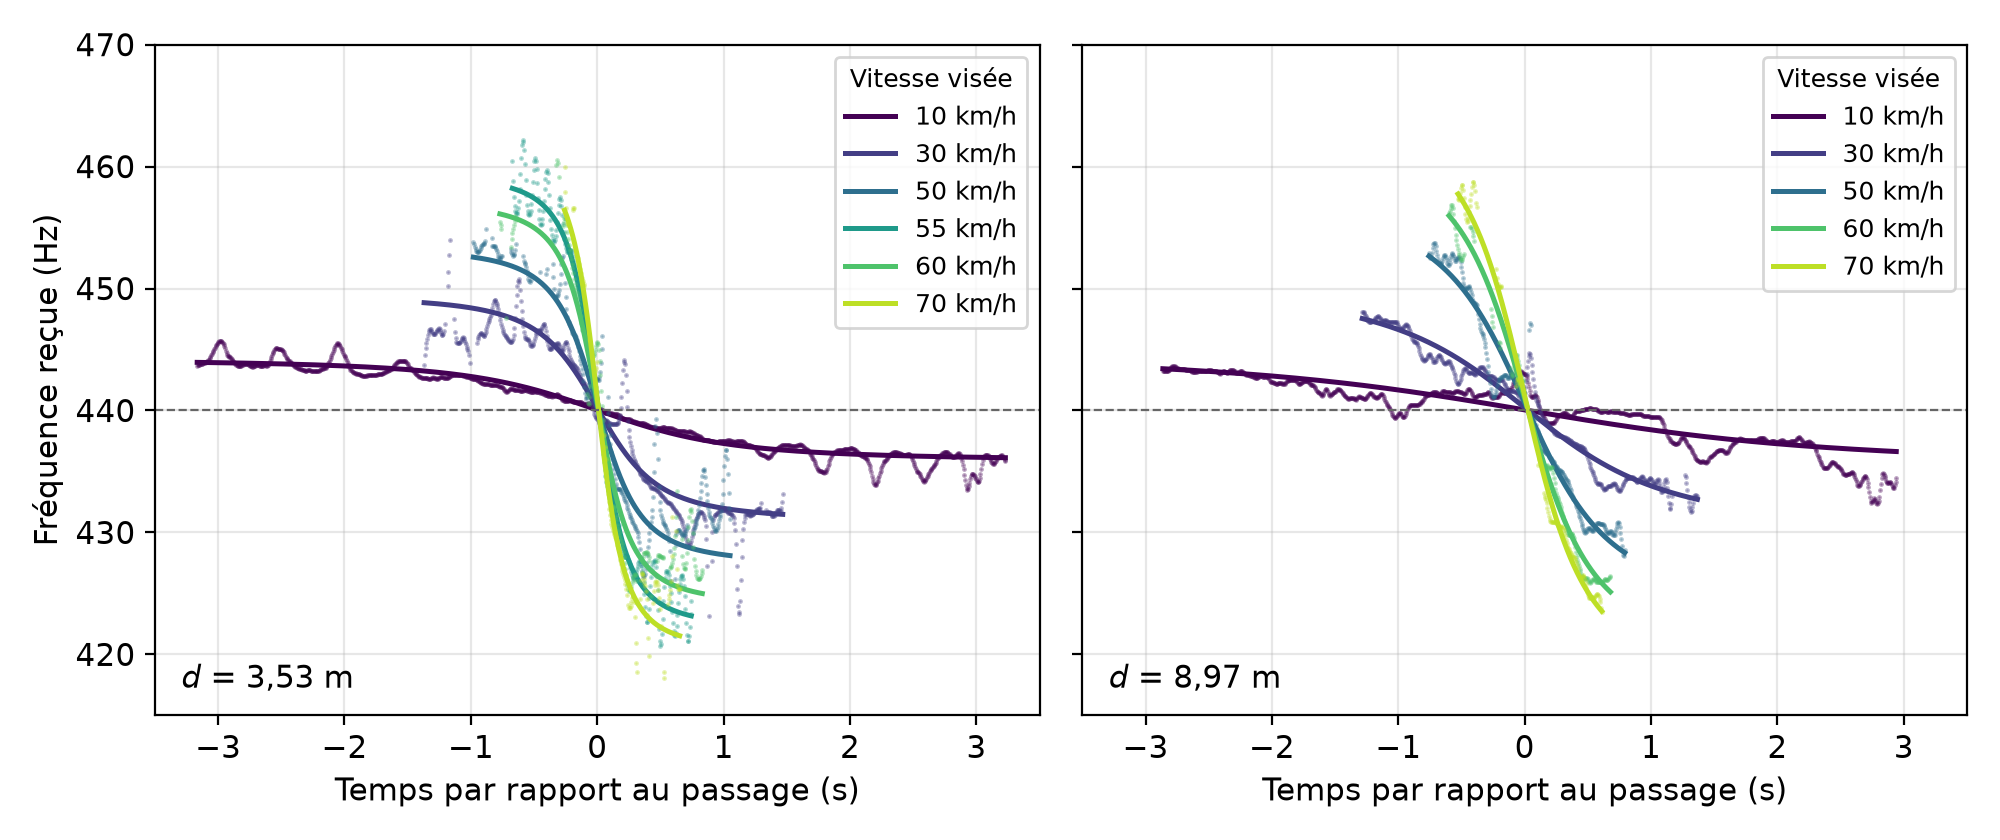
\includegraphics[width=0.95\textwidth]{../figures/02_courbes_doppler.png}
    \caption{Fréquence reçue en fonction du temps autour du passage, dans la zone à vitesse constante, à 3,53~m (gauche) et à 8,97~m (droite). Les points sont les fréquences suivies dans le spectrogramme et les lignes le curve fit avec $d$ fixée. La ligne pointillée grise marque la fréquence émise de 440~Hz.}
    \label{fig:courbes}
\end{figure}

Le Tableau~\ref{tab:resultats} donne la vitesse mesurée avec $d$ fixée et la distance trouvée par le curve fit où $d$ est libre. Les vitesses mesurées sont aussi comparées aux vitesses visées à la Figure~\ref{fig:vitesses}. À 10~km/h, la voiture allait un peu plus vite que la vitesse visée. Pour tous les autres passages, elle allait moins vite, de 6 à 11~\% à 8,97~m et de 8 à 30~\% à 3,53~m.

\begin{table}[htbp]
\centering
\caption{Vitesse mesurée (curve fit avec $d$ fixée) et distance mesurée (curve fit avec $d$ libre) pour les 11 passages.}
\label{tab:resultats}
\small
\begin{tabular}{cccc}
\hline
$d$ au ruban (m) & $v$ visée (km/h) & $v$ mesurée (km/h) & $d$ mesurée (m) \\
\hline
3,53 & 10 & $11{,}3 \pm 0{,}3$ & $5{,}3 \pm 1{,}1$ \\
3,53 & 30 & $25{,}0 \pm 1{,}6$ & $2{,}5 \pm 1{,}4$ \\
3,53 & 50 & $35{,}2 \pm 3{,}4$ & $2{,}3 \pm 1{,}5$ \\
3,53 & 55 & $50{,}5 \pm 1{,}8$ & $3{,}2 \pm 1{,}0$ \\
3,53 & 60 & $44{,}8 \pm 6{,}4$ & $1{,}5 \pm 0{,}9$ \\
3,53 & 70 & $55{,}8 \pm 4{,}9$ & $1{,}8 \pm 1{,}1$ \\
\hline
8,97 & 10 & $12{,}4 \pm 0{,}7$ & n.d.$^a$ \\
8,97 & 30 & $27{,}1 \pm 0{,}8$ & $9{,}5 \pm 6{,}9$ \\
8,97 & 50 & $45{,}0 \pm 1{,}9$ & n.d.$^a$ \\
8,97 & 60 & $56{,}3 \pm 2{,}0$ & n.d.$^a$ \\
8,97 & 70 & $62{,}6 \pm 1{,}6$ & $7{,}1 \pm 2{,}7$ \\
\hline
\end{tabular}
\\[0.3em]
{\footnotesize $^a$ non déterminée: le curve fit ne converge pas et $d$ part vers la limite permise de 30~m.}
\end{table}

\begin{figure}[htbp]
    \centering
    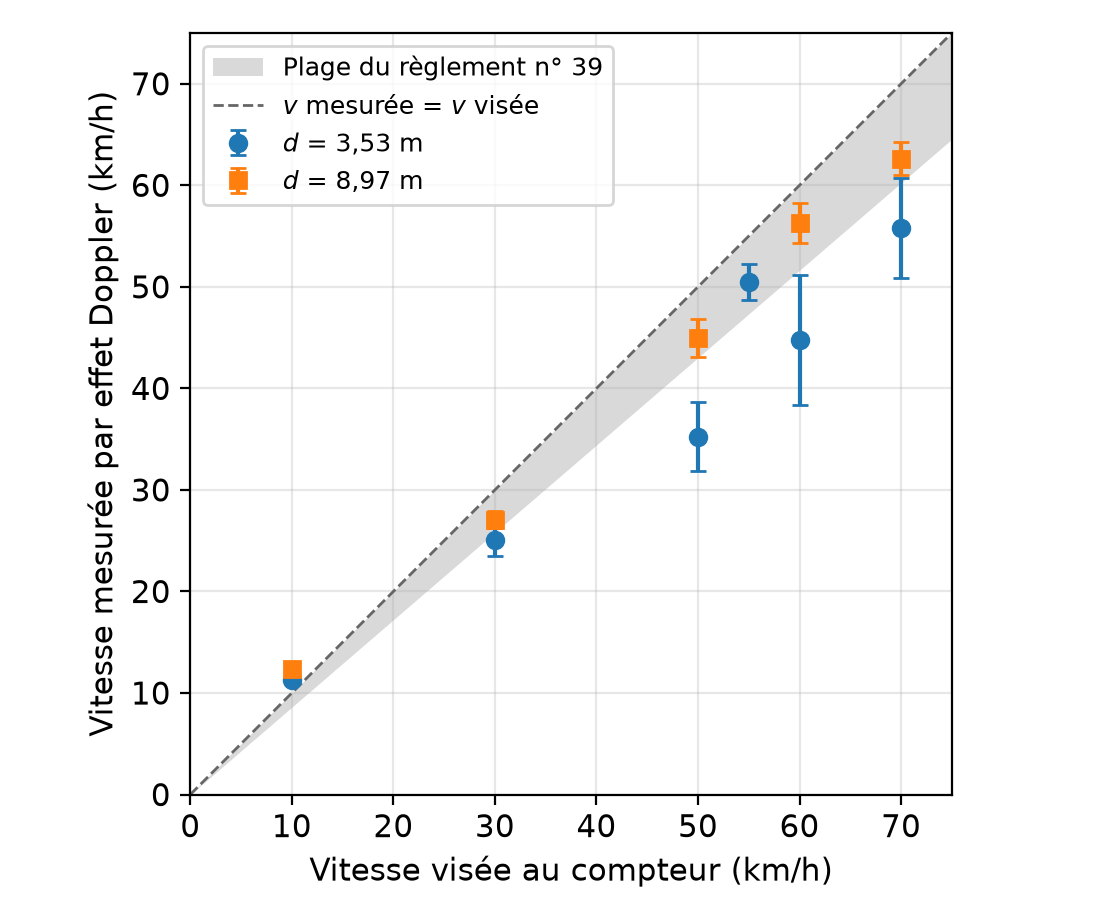
\includegraphics[width=0.5\textwidth]{../figures/03_vitesses.png}
    \caption{Vitesse mesurée par effet Doppler en fonction de la vitesse visée au compteur. La zone grise est la plage de vitesses réelles permise pour un compteur par le règlement n\textsuperscript{o}~39 de la CEE-ONU. À 8,97~m, les passages de 30 à 70~km/h tombent tous dans cette zone.}
    \label{fig:vitesses}
\end{figure}

\section{Discussion}
\label{sec:discussion}

\subsubsection*{Vitesse}
Un compteur de vitesse n'est pas exact. Le règlement n\textsuperscript{o}~39 de la CEE-ONU exige que la vitesse affichée ne soit jamais plus petite que la vitesse réelle, et qu'elle la dépasse d'au plus 10~\% plus 4~km/h \cite{ece39}. À 70~km/h affichés, la voiture peut donc rouler entre 60 et 70~km/h. À 8,97~m, les quatre passages de 30 à 70~km/h tombent dans cette plage (Figure~\ref{fig:vitesses}). L'écart entre la vitesse visée et la vitesse mesurée correspond donc à l'erreur normale d'un compteur, si celui de la voiture suit une règle semblable. À 10~km/h, la voiture allait plus vite que la vitesse affichée, ce qui est impossible selon cette règle. Par contre, l'aiguille est difficile à garder exactement à 10~km/h, et une petite variation de vitesse est déjà 10~\% de la vitesse visée.

À 3,53~m, les passages à 50, 60 et 70~km/h sont sous la zone grise. Ce n'est pas un effet de l'incertitude sur la température, qui ne compte que pour 0,2~\% de $v$. Deux causes peuvent l'expliquer. Premièrement, la position de la source. Les haut-parleurs du système de son sont dans l'habitacle, alors que $d$ est mesurée jusqu'au côté de la voiture. Si la source se trouve en moyenne au centre de la voiture, à environ 0,9~m de son côté, la vraie distance est plus grande que celle utilisée dans le curve fit. Avec $d = 4{,}43~\text{m}$, les vitesses mesurées à 3,53~m augmentent de 0,7 à 7~km/h, contre 0,4 à 2,5~km/h à 8,97~m, où 0,9~m est une plus petite partie de la distance. Cet effet réduit l'écart, mais ne l'explique pas au complet pour le passage à 50~km/h ($37{,}5$~km/h avec $d = 4{,}43~\text{m}$). Deuxièmement, la vitesse n'était probablement pas constante devant le micro. À 3,53~m, la chute de fréquence dure seulement quelques dixièmes de seconde, et la zone à vitesse constante ne compte que 105 à 278 points à 50, 60 et 70~km/h, contre plus de 1000 à 10~km/h. Si la voiture accélère encore en entrant dans la zone ou freine déjà en sortant, la fréquence avant le passage est plus basse et celle après le passage est plus haute que prévu, et le curve fit donne une vitesse trop petite.

\subsubsection*{Distance}
Avec l'audio seulement, la distance est mal déterminée. À 3,53~m, les six distances trouvées vont de 1,5 à 5,3~m. Cinq des six correspondent à 3,53~m à moins de deux fois leur incertitude, qui est d'environ 1~m. La distance est donc connue à environ 30~\% près pour un seul passage. Les distances de 1,5 et 1,8~m, à 60 et 70~km/h, restent sous 3,53~m même en ajoutant leur incertitude. Ce n'est pas possible, parce que la source est dans la voiture et donc au moins à 3,53~m du micro. Elles appuient l'idée que la vitesse n'était pas constante pendant ces passages: une voiture qui freine juste après le point $P$ donne une chute plus courte, qui ressemble à celle d'une voiture qui passe plus près.

À 8,97~m, le curve fit ne converge pas pour trois passages sur cinq. La cause est la longueur de la zone à vitesse constante. Au bord de cette zone ($L = 10~\text{m}$), $\cos\theta$ vaut 0,94 à 3,53~m, mais seulement 0,74 à 8,97~m. À 8,97~m, la fréquence est donc encore loin de $f_a$ et de $f_e$, et on ne voit que la partie centrale de la courbe. Dans cette partie, la fréquence descend presque en ligne droite, avec une pente qui dépend seulement de $v^2/d$ (équation~\ref{eq:pente}). Une voiture plus rapide qui passe plus loin donne donc presque la même courbe, et le curve fit ne peut pas les séparer. Pour avoir $\cos\theta = 0{,}95$ au bord de la zone à 8,97~m, il faudrait une vitesse constante sur $|x| \leq 3d \approx 27~\text{m}$, soit environ 55~m au total.

\subsubsection*{Dispersion près du passage}
À 3,53~m, la fréquence suivie est beaucoup plus dispersée autour du curve fit juste après le passage (Figure~\ref{fig:courbes}). Le bruit du moteur et des pneus y est le plus fort (Figure~\ref{fig:spectro}), ce qui diminue le rapport signal sur bruit. Aussi, le son arrive au micro par plusieurs chemins: les haut-parleurs sont à différents endroits dans la voiture et le son se réfléchit sur la route. Proche du point $P$, chaque chemin a un angle $\theta$ différent et donc un décalage Doppler différent, et ces sons interfèrent. Cet effet est plus fort quand la voiture passe proche du micro, parce que les angles changent plus vite.

\subsubsection*{Améliorations}
La principale amélioration serait une zone à vitesse constante plus longue, d'au moins 50~m, avec le régulateur de vitesse. Aussi, la vitesse réelle de chaque passage pourrait être mesurée avec le GPS d'un cellulaire dans la voiture pour avoir une valeur de référence plus précise que le compteur. Un petit haut-parleur fixé à l'extérieur, sur le côté de la voiture, donnerait une seule source à une position connue. Faire plusieurs passages pour chaque vitesse permettrait de vérifier si les résultats se répètent, alors qu'il n'y en a eu qu'un ici.

\section{Conclusion}
\label{sec:conclusion}

Un sinus de 440~Hz joué par le système de son d'une voiture a permis de mesurer la courbe Doppler de 11 passages, à 3,53 et 8,97~m d'un sonomètre. La vitesse change la hauteur de la chute de fréquence et la distance change sa durée, comme le prévoit le modèle. Quand la distance est connue, un seul passage suffit pour mesurer la vitesse: à 8,97~m, les vitesses mesurées sont de 6 à 11~\% sous la vitesse affichée au compteur, ce qui correspond à l'erreur permise pour un compteur. À 3,53~m, les passages rapides sont plus lents que prévu, probablement à cause de la position de la source dans la voiture et d'une vitesse qui n'était pas tout à fait constante. Retrouver aussi la distance avec l'audio seulement n'a fonctionné qu'à 3,53~m, à environ 1~m près. Pour répondre au deuxième objectif, une prochaine expérience devrait garder la vitesse constante sur au moins 50~m, pour que la fréquence atteigne ses valeurs d'approche et d'éloignement. Aussi, mesurer la vitesse de référence avec un GPS permettrait de vérifier la précision de la méthode sans dépendre du compteur.

\renewcommand{\refname}{Bibliographie}
\begin{thebibliography}{9}

\refsicitee{protocole}{%
Département de physique, de génie physique et d'optique, Université Laval. \textit{GPH-3000, Travaux pratiques avancés: Acoustique}, protocole, automne 2022.}

\refsicitee{doppler}{%
Doppler, C. « Über das farbige Licht der Doppelsterne und einiger anderer Gestirne des Himmels ». \textit{Abhandlungen der Königlichen Böhmischen Gesellschaft der Wissenschaften}, 5\textsuperscript{e} série, vol.~2, p.~465-482, 1842.}

\refsicitee{buysballot}{%
Buys Ballot, C.H.D. « Akustische Versuche auf der Niederländischen Eisenbahn, nebst gelegentlichen Bemerkungen zur Theorie des Hrn. Prof. Doppler ». \textit{Annalen der Physik und Chemie}, vol.~142, n\textsuperscript{o}~11, p.~321-351, 1845.}

\refsicitee{morse}{%
Morse, P.M. et Ingard, K.U. \textit{Theoretical Acoustics}. McGraw-Hill, New York, 1968.}

\refsicitee{kinsler}{%
Kinsler, L.E., Frey, A.R., Coppens, A.B. et Sanders, J.V. \textit{Fundamentals of Acoustics}, 4\textsuperscript{e} édition. Wiley, New York, 2000.}

\refsicitee{ece39}{%
Commission économique des Nations Unies pour l'Europe (CEE-ONU). \textit{Règlement n\textsuperscript{o}~39: Prescriptions uniformes relatives à l'homologation des véhicules en ce qui concerne l'appareil indicateur de vitesse, y compris son installation}. Genève.}

\refsicitee{guier}{%
Guier, W.H. et Weiffenbach, G.C. « Genesis of Satellite Navigation ». \textit{Johns Hopkins APL Technical Digest}, vol.~19, n\textsuperscript{o}~1, p.~14-17, 1998.}

\end{thebibliography}

\end{document}
